Este capítulo aborda la metodología utilizada por los Sistemas Windows para desarrollar la autenticación y posterior autorización de un usuario u objeto. Con este fin, se pro\-fun\-di\-za\-rá en el inicio de sesión interactivo, independientemente de si es de forma local o remoto, la gestión de las credenciales introducidas por el usuario hasta su posterior validación y finalmente, la comprobación de si ese usuario u objeto tiene permisos suficientes para ejecutar la acción que está solicitando. 

\section{Autenticación vs autorización}

La mayoría de ataques y vulnerabilidades que amenazan Sistemas Windows y por consecuencia Active Directory utilizan debilidades en los procesos de autenticación y autorización de estos. Por lo tanto, es importante conocer los procesos y procedimientos involucrados así como las diferencias entre autenticación y autorización~\cite{Capitulo2:AuthenticationConcepts}: \\

Por un lado, la autenticación consiste en la verificación de la identidad de un usuario, dicho con otras palabras, que el sistema de autenticación, como puede ser a la hora de iniciar sesión, asegure que el usuario es quien dice ser. Esta verificación se puede realizar, por ejemplo, con un secreto o contraseña conocido únicamente por el usuario y que será validada posteriormente. \\

Por otro lado, cuando se habla de autorización se refiere a establecer y delimitar qué recursos son a los que puede acceder el usuario en cuestión o grupos de usuarios. Por ejemplo, establecer que los usuarios administradores puedan acceder a carpetas compartidas con información confidencial. La verificación de que un usuario puede realizar la acción que está solicitando realizar, como puede ser el acceso a un dispositivo, recurso, etc. 


\section{Escenarios de autenticación}

Para utilizar equipos basados en Windows es necesario disponer de una cuenta válida independientemente de si se solicita acceder a un equipo localmente o en red. Por lo tanto, Windows provee tecnología de control de acceso para determinar tanto si un usuario es quién dices ser, es decir, el proceso de autenticación como para gestionar  si dicho usuario tiene los permisos necesarios para acceder al recurso o dispositivo que está solictando. A continuación se va a enumerar los posibles casos en los que se solicitará la autenticación de un usuario~\cite{Capitulo2:Scenarios}:

\subsection{Inicio de sesión interactivo (interactive logon)}

Este escenario corresponde al inicio de sesión principal en sistemas basados en Windows por lo que se detallará en las secciones siguiente de este capítulo. Ocurre cuando un usuario accede a una cuenta de usuario local o a una cuenta de dominio para iniciar sesión en un equipo. \\

Se produce un inicio de sesión de forma local cuando un usuario tiene acceso físico al equipo y este no está unido a ningún dominio o cuenta de usuario en Active Directory. Este inicio de sesión requiere disponer de una cuenta de usuario en el administrador de cuentas de seguridad del inglés {\it Security Account Manager (SAM)} donde se comprobará si las credenciales almacenadas son iguales a las credenciales proporcionadas por el usuario. Este inicio de sesión permite acceder al usuario a los recursos de Windows del equipo local. \\

Inicio de sesión en dominio ocurre cuando un usuario accede a una cuenta de usuario en Active Directry. Para ello, es necesario que el equipo disponga de una cuenta de dominio de Active Directory y esté conectado físicamente a la red. Esto le permite tener acceso tanto a los recursos locales como los recursos proporcionados por el dominio (carpetas compartidas, servicios, etc.). \\

Además, también se produce  un inicio de sesión interactivo cuando un usuario accede de manera remota a un equipo a través del protocolo de escritorio remoto del inglés {\it Remote Desktop Protocol (RDP)}. Las credenciales son enviadas al equipo donde se está intentado conectar y este es el que procede a su posterior validación. 

\subsection{Inicio de sesión a través de aplicaciones o servicios}

Este escenario ocurre cuando una aplicación o un servicio solicita que un usuario inicie sesión para acceder a los recursos que ofrece dicha aplicación o servicio. Como se puede observar en la Figura \ref{RunAs}, al ejecutar el comando RunAs que lanza la aplicación {\it cmd.exe} como el usuario {\it Cliente01}, este nos solicita la contraseña de dicho usuario. Además, Windows gestiona las credenciales para aplicaciones y servicios que no requieren la interacción de un usuario. \\

Los sistemas basados en Windows, implementan inicio de sesión único conocido como {\it Single Sign-On (SSO)}~\cite{Capitulo2:SingleSignOn}. El objetivo principal de SSO es que sólo haya que introducir las credenciales de un usuario una única vez para acceder a cualquier recurso que necesite autenticación (en vez de introducir las credenciales cada vez). Como se verá a continuación, Windows guarda de manera local en memoria dichas credenciales en el subsistema {\it Local Security Authority (LSA)}.

\begin{figure}[t!] %[ht!] para here [b] para bottom [t] para top
\begin{center}
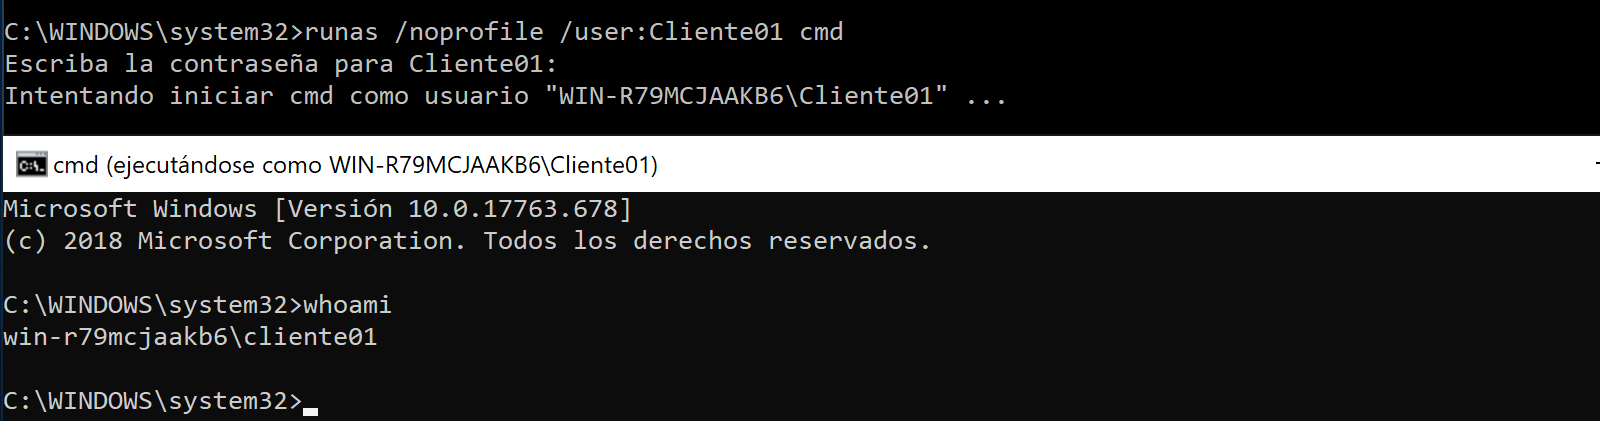
\includegraphics[width=16cm]{Runas.png}
\end{center}
\caption{Autenticación al ejecutar el comando RunAs.}
\label{RunAs}
\end{figure}

\subsection{Inicio de sesión en red}

El inicio de sesión en red del inglés {\it Network Logon} ocurre una vez el usuario es correctamente autenticado en un equipo a través de alguno de los procesos explicados anteriormente e intenta acceder a cualquier servicio de red. Este proceso suele ser invisible al usuario a no ser que sean necesarias otras credenciales. 

\subsection{Otros escenarios}

Existen otros escenarios de inicio de sesión como puede ser ``Inicio de sesión a través de Smartcard'' que requiere el uso del protocolo Kerberos o ``Inicio de Sesión biométrico'' donde se utiliza un dispositivo para obtener las credenciales biométricas, como puede ser la huella digital, y se comparan con las credenciales almacenadas durante la creación de la cuenta.  

\section{Inicio de sesión interactivo}

El proceso de autenticación a través de inicio de sesión interactivo, del inglés {\it Interactive Logon}, a diferencia del inicio de sesión en red o {\it Network Logon}, es llevado a cabo por el proceso {\it WinLogon} que se encarga de recoger las credenciales introducidas por el usuario y su posterior validación. Un usuario que inicia sesión en un equipo ya sea localmente o un inicio de sesión en red introduce el usuario y la contraseña (denominado credenciales de usuario) y sirve para verificar la identidad del usuario. Por otro lado, cuando se inicia sesión a través de una Smart Card {\it (Smart Card Logon)} las credenciales están almacenadas en el chip de la tarjeta y estas son leídas por un dispositivo externo y el usuario introduce el {\it Personal Identification Number (PIN)}.\\

\subsection{Proceso de inicio de sesión interactivo (WinLogon)}

{\it WinLogon.exe} es el proceso encargado de coordinar y administrar el inicio de sesión interactivo. Además, este proceso también se encarga de gestionar el {\it logout}, lanzar los procesos necesarios para la autenticación de un usuario, cambiar las contraseñas, bloquear y desbloquear un equipo y proporcionar la seguridad necesaria para que ningún otro proceso pueda acceder a información sensible cuando estos procedimientos se están llevando a cabo. \\

Como se puede ver en la Figura \ref{WinLogon} el proceso de inicio interativo consta de varias fases~\cite{Capitulo2:WinInternals}:

\begin{figure}[t!] %[ht!] para here [b] para bottom [t] para top
\begin{center}
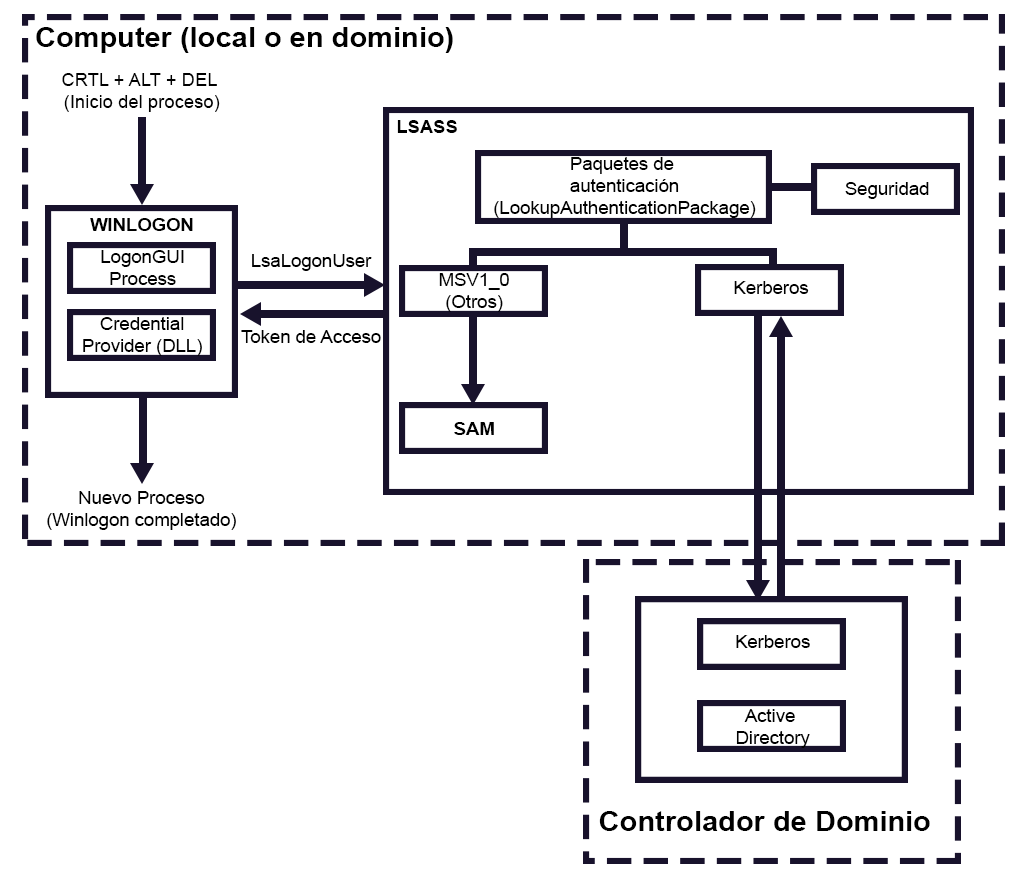
\includegraphics[width=16cm]{WinLogon.png}
\end{center}
\caption{Proceso de inicio de sesión interactivo (WinLogon).}
\label{WinLogon}
\end{figure}

\begin{enumerate}
\item En primer lugar, el proceso de inicio de sesión comienza con una secuencia denominada {\it Secure Attention Sequence (SAS)}. Esta secuencia es {\it CTRL + ALT + DEL} por defecto e inicia el proceso {\it WinLogon.exe}.

\item {\it WinLogon.exe} es el ejecutable encargado de gestionar el inicio de sesión interactivo. Para ello, inicializa el proceso {\it LogonUI.exe} cuya finalidad es proporcionar la interfaz de usuario por defecto y recoger las credenciales introducidas. 

\item {\it LogonUI.exe} es el proceso encargado de solicitar, enumerar y mostrar al usuario la interfaz con las credenciales necesarias para la autenticación. Para ello, consulta los diferentes {\it Credential Providers}~\cite{Capitulo2:CredentialProviders} de los que dispone el sistema. Los {\it Credential Providers} son bibliotecas de enlace dinámico, del inglés {\it Dynamic-Link Library (DLL)}, que se encargan de proporcionar la información necesaria, manejar la co\-mu\-ni\-ca\-ción y la lógica con las entidades de autenticación externas y serializar y empaquetar las credenciales correctamente. Estas DLLs se encuentran en \footnote{\%SystemRoot\%\textbackslash{}System32\textbackslash{}authui.dll} o en \footnote{\%SystemRoot\%\textbackslash{}System32\textbackslash{}SmartcardCredentialProvider.dll} (Si se trata de un inicio de sesión con Smart Cards).

\item Una vez introducidas las credenciales, {WinLogon.exe} se comunica con el proceso LSASS a través de la función {\it LsaLookupAuthenticationPackage}. Esta función tiene como objetivo obtener los paquetes de autenticación disponibles en el sistema a través de la clave de registro \footnote{HKEY\_LOCAL\_MACHINE\textbackslash{}SYSTEM\textbackslash{}CurrentControlSet\textbackslash{}Control\textbackslash{}Lsa} como se puede observar en la Figura \ref{Registro-Auth}.

\begin{figure}[t!] %[ht!] para here [b] para bottom [t] para top
\begin{center}
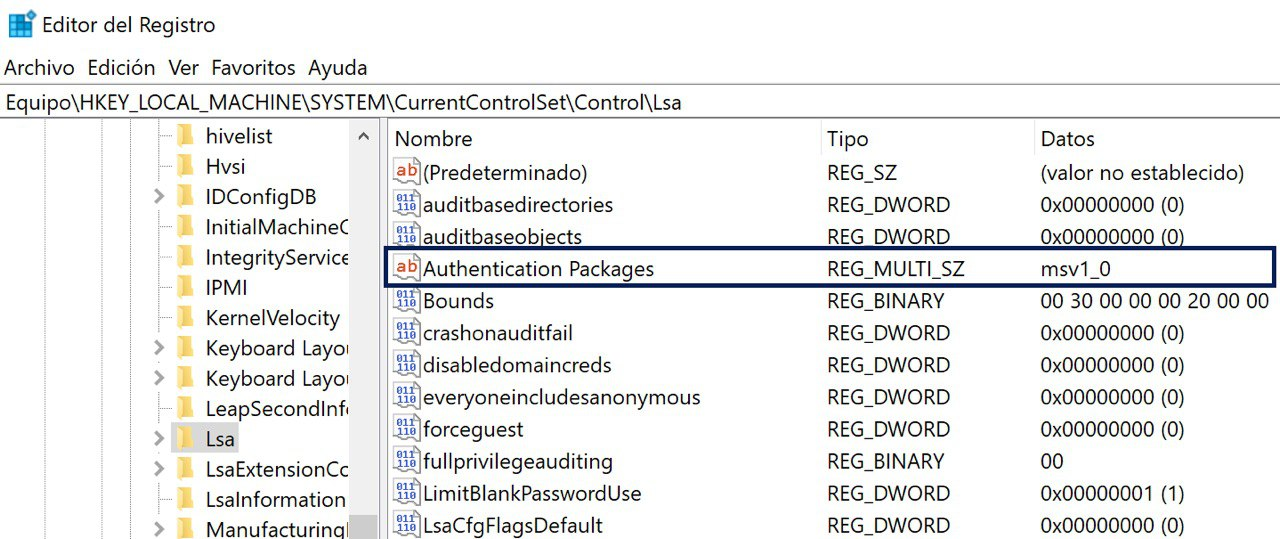
\includegraphics[width=16cm]{Registro-Auth.jpg}
\end{center}
\caption{Clave de registro sobre los paquetes de autenticación.}
\label{Registro-Auth}
\end{figure}

\item Posteriormente, se envían las credendiales a través de la función {\it LsaLogonUser}. Si algún paquete de autenticación autentica al usuario el proceso continua, en cambio, si ningún paquete indica que se ha iniciado sesión correctamente el proceso acaba. Los paquetes de autenticación usados por Windows por defecto son MSV1\_0 y Kerberos, ambos se detallarán en el siguiente capítulo de la literatura. 

\item Cuando se trata de un inicio de sesión en dominio, LSA utiliza el proceso {\it Netlogon.exe}, este proceso se encarga de mantener un canal de comunicación seguro entre el equipo y el controlador de dominio ({\it Domain Controller}) y de pasar las credenciales a través de este. 

\item Una vez autenticado, el proceso LSASS comprobará en la base de datos de políticas locales si el usuario autenticado tiene los permisos suficientes para realizar la acción que está solicitando. Si el inicio de sesión no coincide el proceso de autenticación acaba y LSASS elimina cualquier estructura de datos creada y lo notifica a WinLogon. Si el acceso está permitido, LSASS agrega los IDs de seguridad correspondientes, busca en la base de datos los permisos asociados a los usuarios del mismo grupo del SID del usuario, los añade al token de acceso ({\it Access Token}) y crea dicho token que será enviado a Winlogon con un mensaje de inicio de sesión correcto. 

\item Por último, Winlogon mira en el registro \footnote{HKLM\textbackslash{}SOFTWARE\textbackslash{}Microsoft\textbackslash{}Windows NT\textbackslash{}Current Version\textbackslash{}Winlogon\textbackslash{}Userinit} y crea un proceso con el valor que haya contenido en el registro. El valor por defecto es {\it Userinit.exe} que carga el perfil del usuario autenticado. 

\end{enumerate}

Una vez definido el proceso de inicio interactivo a grandes rasgos, se va a pasar a detallar los componentes mencionados que forman parte de dicho proceso.

\subsection{Local Security Authority (LSA)}

{\it Local Security Authority}~\cite{Capitulo2:LSA} se encarga de validar el acceso a los objetos, comprobar si un usuario tiene permisos suficientes y generar mensajes de auditoría. Es decir, LSA se encarga de las siguientes acciones:

\begin{itemize}
\item Autenticar y registrar los usuarios en un sistema local, es decir, se encarga del proceso visto anteriormente. 
\item Administrar la politica de seguridad local de un sistema, del inglés {\it Local Security Policy}.
\item Proporcionar los servicios necesarios tanto para la autenticación de un usuario, como para la generación de los tokens de acceso correspondientes.
\item Gestionar los servicios necesarios para mantener la relación entre nombres y SIDs.
\end{itemize}

\subsubsection{Local Security Authority Subsystem Service (LSASS)}

El proceso {\it Local Security Authority Subsystem Service (LSASS)} se encarga de instanciar las políticas de seguridad en el sistema, realizar un seguimiento de las políticas de seguridad de las cuentas activas, modificar credenciales y crear tokens de acceso y almacenar las credenciales de los usuarios activos del sistema. Esto permite que un usuario no tenga que introducir las credenciales cada vez que accede a un recurso {\it (Single Sign-On)}~\cite{Capitulo2:SingleSignOn}.\\

Este proceso es de gran interés para los atacantes ya que LSASS puede almacenar credenciales como Tikets de Kerberos, Hashes NT, Hashes LM o credenciales con algoritmos de cifrado débiles que se puede obtener la contraseña en texto claro.\\

LSASS almacena las credenciales de las sesiones activas, estas credenciales se almacenan cuando un usaurio realiza alguna de las siguientes acciones:

\begin{itemize}
\item Se inicia sesión localmente (o remotamente a través de {\it Remote Desktop Protocol (RDP)}). 
\item Se ejecuta un proceso o tarea usando el comando {\it RunAs}.
\item Se ejecuta un servicio de Windows que necesite mayores privilegios de los actuales y se requiere autenticación.
\item Se ejecuta una tarea programada para la que es necesario autenticarse. 
\item Se ejecuta una tarea local usando una herramienta de administración remota. 
\end{itemize}

\subsubsection{Logon Sessions}

{\it Logon Sessions}~\cite{Capitulo2:LogonSessions}~\cite{Capitulo2:LogonSessions2} es una estructura de datos que representa un {\it Security Principal}~\cite{Capitulo2:SecurityPrincipals}. Una entidad de seguridad del inglés {\it Security Principal} corresponde a cualquier entidad que se puede autenticar en un sistema basado en Windows como puede ser usuarios, grupos de usuarios o procesos ejecutados en un contexto de seguridad de usuarios o grupos de usuarios. \\

Cuando un usuario inicia sesión de forma satisfactoria el proceso LSA crea una {\it Logon Session} que será utilizada para la creación del token de acceso y se incrementará la referencia al número de sesiones creadas. Esta referencia también es aumentada cuando se duplica el token, cuando un usuario ejecuta procesos en nombre de otro usuario, etc. \\

Para listar las  {\it Logon Sessions} en un sistema se puede utilizar el comando {\it logonsessions} de {\it Windows Sysinternals}~\cite{Capitulo2:Sysinternals} como se puede ver en la Figura \ref{Logonsessions}.

\begin{figure}[t!] %[ht!] para here [b] para bottom [t] para top
\begin{center}
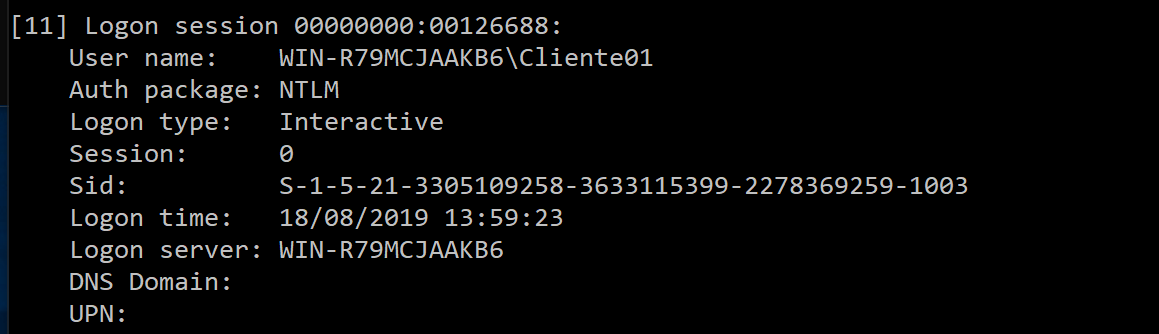
\includegraphics[width=16cm]{Logonsessions.png}
\end{center}
\caption{Salida del comando Logonsessions.}
\label{Logonsessions}
\end{figure}


\subsection{Security Support Provider Interface (SSPI)}

Aunque no se ha mencinado anteriormente, {\it Security Support Provider Interface (SSPI)} ~\cite{Capitulo2:SSPI} es una API que permite que una aplicación pueda utilizar varios modelos de seguridad, es decir, abstrae las llamadas necesarias en el proceso de autenticación y permite que una aplicación lleve a cabo un proceso de autenticación sin especificar los protocolos de autenticación, denominados paquetes de autenticación que se verán en detalle en la siguiente sección de este capítulo.\\

En primer lugar, se negocia el protocolo a utilizar, para que el proceso se complete correctamente ambas máquinas deben aceptar el mismo {\it Security Support Provider (SSP)}. Un SSP es un DLL que implementa SSPI y permite la ejecución de los paquetes de autenticación. Cada paquete proporciona un ``mapeo'' entre las llamadas de funciones SSPI de una aplicación y las funciones de un modelo de seguridad.\\

Los principales SPP son: 

\begin{itemize}

\item Kerberos.
\begin{listing}[style=consola, numbers=none]
%SystemRoot\%\Windows\System32\kerberos.dll
\end{listing}

\item NT Lan Manager (NTLM): NTLMv1 y NTLMv2.
\begin{listing}[style=consola, numbers=none]
%SystemRoot%\Windows\System32\msv1_0dll
\end{listing}

\item Digest.
\begin{listing}[style=consola, numbers=none]
%SystemRoot%\Windows\System32\Wdigest.dll
\end{listing}

\item Schanell.
\begin{listing}[style=consola, numbers=none]
%SystemRoot%\Windows\System32\Schannel.dll
\end{listing}

\item Negotiate.
\begin{listing}[style=consola, numbers=none]
%SystemRoot%\Windows\System32\lsasrv.dll
\end{listing}

\end{itemize}

\subsubsection{Negotiate}

Microsoft Negotiate~\cite{Capitulo2:Negotiate} es un SSP que actúa como intermediario entre la API SPPI y otro SSP. Cuando una aplicación requiera algún tipo de autenticación, se envía una petición a Negotiate con los argumentos necesarios (parámetros, credenciales, SSPs a utilizar...), este lo examinará y pasará la petición al SSP correspondiente que llevará a cabo la autenticación. \\

Actualmente, Negotiate elige entre Kerberos y NTLM. Seleccionará el primero siempre y cuando haya conexión entre las dos partes implicadas en el proceso y el usuario haya especificado el Service Principal Name (SPN), un User Principal Name (UPN), o una cuenta de NetBIOS. En cambio, si se trata de una autenticación local utilizará NTLM.

\subsection{Security Account Manager (SAM)}

{\it Security Account Manager (SAM)} corresponde a una base de datos que almacena localmente la información sobre las cuentas de usuario y grupos de usuarios (identificador de usuario, nombre de usuario y hash de la contraseña). Esta información es consultada por el proceso LSA a la hora de autenticar a un usuario de forma local comparando el hash de la contraseña introducida por el usuario y el hash de la contraseña contenido en base de datos SAM. Esta base de datos corresponde con el fichero: 

\begin{listing}[style=consola, numbers=none]
%SystemRoot%\Windows\System32\config\SAM
\end{listing}

\section{Autorización}

Una vez completado correctamente el proceso de autenticación, se procede a comprobar si el usuario tiene los privilegios necesarios para realizar la acción que se está solicitando ejecutar, como puede ser acceder a un equipo, acceder a un recurso, etc. 


\subsection{Access tokens}

Cuando el proceso LSA verifica la autenticación del usuario, se crea un {\it Access Token}, este objeto describe el contexto de seguridad de un proceso o de un hilo ({\it thread})~\cite{Capitulo2:Access-Token}. Para los SSPI se denomina contexto de seguridad a una estructura de datos que contiene datos relevantes de seguridad como puede ser la clave de sesión o la duración de dicha sesión. Cada proceso ejecutado por un usuario dispone de una copia del token de acceso de ese usuario. Windows utiliza estos tokens para identificar a un usuario cuando ejecuta un hilo que necesite privilegios de ese usuario. La información contenida en un {\it Access Token} es:

\begin{itemize}
\item El SID de la cuenta del usuario en cuestión.
\item El SID del grupo de usuarios de los que el usuario es miembro.
\item El SID de la session (logon session).
\item Los privilegios del usuario y del grupo de usuarios al que pertenece.
\item El SID del grupo primario. 
\item El {\it Discretionary Access Control List} (DACL)~\cite{Capitulo2:DACL} por defecto que se utiliza cuando el usuario crea un proceso sin especificar el descriptor de seguridad.
\item La procedencia del token de acceso.
\item Si el token de acceso es primario o es una suplantación. 
\item Una lista de SIDs restrictivos.
\item Niveles de suplatación actuales.
\item Otras estadísticas. 
\end{itemize}

Cuando un administrador local inicia sesión en una máquina, se crean dos tokens diferentes: Un token primario que contendrá el contexto de seguridad del usuario y un token de administrador. Esto es debido a la política de Windows de mínimo privilegio posible, esto significa que el sistema usará por defecto el token primario cuando un proceso o hilo interactue con un {\it Securable Objects}~\cite{Capitulo2:Securable-Objects}. Esto es importante a la hora de entender {\it User Account Control (UAC)}.\\

\subsection{User Account Control (UAC)}

User Account Control (UAC)~\cite{Capitulo2:UAC}~\cite{Capitulo2:UAC2}sirve para controlar cuando se están usando privilegios de administración. Como se ha comentado anteriormente al iniciar sesión desde una cuenta administrativa, se crean dos tokens de usuario: uno denominado {\it full access token} y un token secundario denominado {\it filtered access token}. Esto permite que los procesos ejecutados por este usuario se ejecuten con el segundo token siempre y cuando no necesiten privilegios de administración y así cumplir la política de mínimo privilegio posible. Esto lo podemos observar cuando se completa un inicio de sesión válido, el proceso {\it Explorer.exe} se ejecuta con el {\it filtered access token}. Cuando un proceso concreto necesita privilegios de administración, se requerirá una elevación de privilegios realizando una elevación de UAC. Como se puede ver en la Figura \ref{UAC} se ha ejecutado una terminal {\it (cmd.exe)} con privilegios administrativos y aparece el mensaje de Control de Cuentas de Usuario para elevar de privilegios. \\

\begin{figure}[t!] %[ht!] para here [b] para bottom [t] para top
\begin{center}
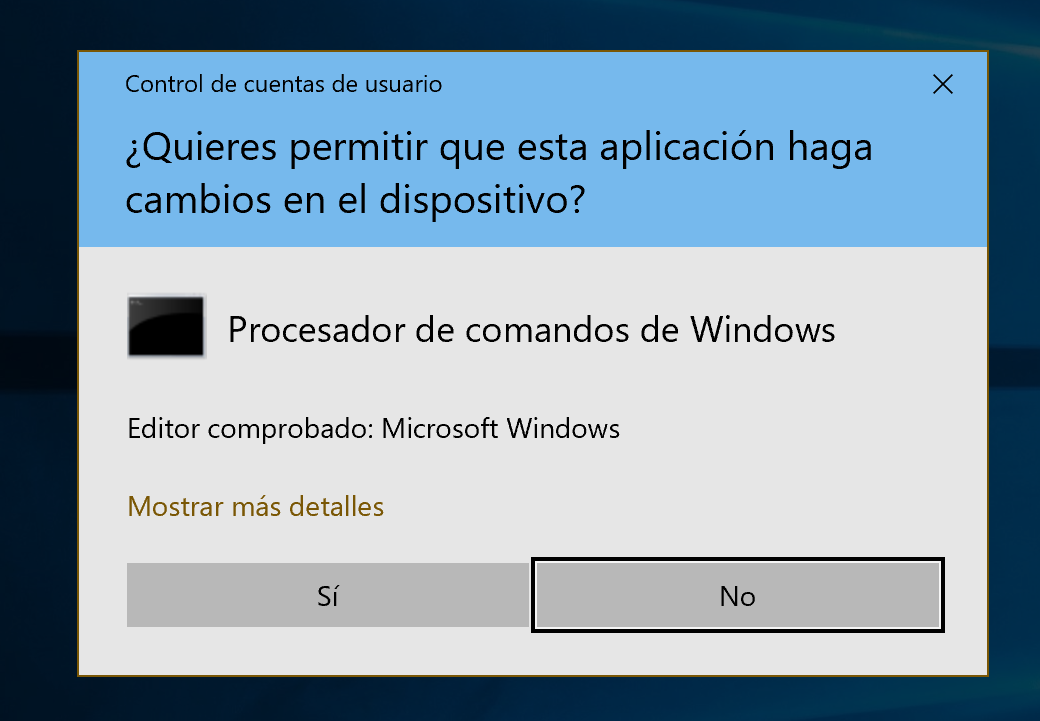
\includegraphics[width=10cm]{UAC.png}
\end{center}
\caption{Control de Cuentas de Usuario al ejecutar cmd.exe}
\label{UAC}
\end{figure}

Para controlar qué procesos necesitan privilegios especiales o cuales no, los Sistemas Windows hacen uso de {\it Mandatory Integrity Control}~\cite{Capitulo2:MIC}, un mecanismo para controlar el acceso a los {\it Securable Objects}~\cite{Capitulo2:Securable-Objects}, para ello, el MIC utiliza niveles de integridad para evaluar el acceso a un proceso. Estos niveles son: {\it untrusted, low, medium, high, system e installer}~\cite{Capitulo2:IntegrityLabels}~\cite{Capitulo2:IntegrityLabels2}. Esto implica que un objeto con integridad baja (low) no puede escribir en un objeto de integridad medio. \\

\begin{itemize}
\item \textbf{Untrusted:} Son aquellos procesos iniciados de forma anónima, como puede ser procesos lanzados desde cuentas de invitados.  
\item \textbf{Low:} Nivel de integridad usado por defecto para la interacción con internet. Cuando se lanza {\it Internet Explorer} se utiliza este modo, por lo tanto, todos los archivos y procesos asociados a este se le asignan un nivel de integridad bajo.
\item \textbf{Medium:} Nivel de integridad usado por la mayoría de los procesos, es el nivel designado por defecto siempre y cuando no se especifique explícitamente un nivel inferior o superior.
\item \textbf{High:} Nivel de integridad destinado para aquellos procesos que necesitan privilegios de administración. Los objetos con este nivel de integridad solicitarán una elevación de privilegios a través de UAC.
\item \textbf{System:} Nivel de integridad reservado para los objetos del sistema, estos objetos engloban el kernel de Windows y servicios del {\it core}.
\item \textbf{Installer:} Nivel de integridad especial utilizado para la instalación de software. Este nivel es igual o superior a todos los niveles anteiores, lo que permite que este nivel puede desinstalar los demás objetos. 
\end{itemize}
